\chapter{Implementation}
\label{chap:implementation}
\section{Traffic Manager}
A custom developed Traffic Manger will be used to simulate an traffic environment, which can subsequently be controlled by the Genetic Algorithm. The Traffic Manager is not part of the master's thesis and will be regarded as a "blackbox", only receiving a brief introduction.
Generally speaking, it will simulate traffic using a start scenario, in which the positions and types of actors (vehicles and pedestrians) are defined. 
A simulation always consist of at least one EGO vehicle. Additionally any number of NPCs can be added.

While the NPCs are only controlled by the Traffic Manager, the EGO vehicle can be either partly or completely supervised by an ADAS/AD function. The goal of the genetic algorithm is subsequently to test this function for safety, comfort etc... by controlling the NPCs in order to generate critical scenarios.

For all simulations done by this thesis, the Traffic Manager was set to 100Hz and the simulation duration set to 35 seconds.

\subsection{Action Interface}
\label{implementation:action_interface}
In order to control the behaviour of all actors inside the simulation, actions can be requested over the Action Interface, which is provided by the Traffic Manager. An action will initiate a certain behaviour from an actor and can be set at any timestep\footnote{depending on the ADAS/AD function under test, the Action Interface might be disabled for the EGO vehicle}. Pedestrians and vehicles have a different set of possible actions. If no action is applied, the actor will behave in a normal manner inside the simulation. This means that the actor will follow along its given path until a new action changes its behaviour.

The following list shows all actions provided by the traffic manager which were available for the genetic algorithm at the time of this master's thesis.
\begin{itemize}
	\item JunctionSelection
	\begin{itemize}
		\item vehicle\_id: int, step: int, junction\_selection\_angle (radiants): float
		\item Vehicles will chose which direction to take at junctions based on this angle.
	\end{itemize}
	\item LaneChange
	\begin{itemize}
		\item vehicle\_id: int, step: int, direction: float, distance: float, delay (optional): float
		\item Initiates a lane-change based on its given parameters.
	\end{itemize}
	\item AbortLaneChange
	\begin{itemize}
		\item vehicle\_id: int, step: int
		\item Will abort a current lane-change.
	\end{itemize}
	\item ModifyTargetVelocity
	\begin{itemize}
		\item vehicle\_id: int, step: int, percentage: float
		\item Modifies the internal target velocity of the vehicle by a percentage. If set to 0, the vehicle will stop.
	\end{itemize}
	\item TurnHeading
	\begin{itemize}
		\item pedestrian\_id: int, step: int
		\item The pedestrian will turn 180 degrees and walk in the opposite direction
	\end{itemize}
	\item CrossRoad
	\begin{itemize}
		\item pedestrian\_id: int, step: int
		\item The pedestrian will cross the road immediately.
	\end{itemize}
	\item CrossAtCrosswalk
	\begin{itemize}
		\item pedestrian\_id: int, step: int
		\item The pedestrian will cross the road at the next crosswalk.
	\end{itemize}
\end{itemize}

The genetic algorithm will control only NPCs, a behaviour tree is used for the EGO vehicle itself. Both methods use the Action Interface to control their respective actors. An overview is provided in figure \ref{figure:traffic_manager:structure}.

\begin{figure}[ht] 
	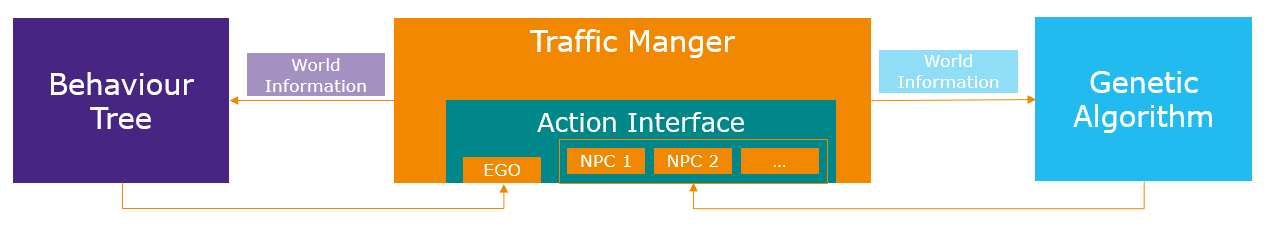
\includegraphics[width=1\linewidth]{figures/tm_structure}
	\caption{Action Interface Structure}
	\label{figure:traffic_manager:structure}
\end{figure}

\section{Genetic Algorithm}
The genetic algorithm will search for sequences of actions that will result in the most interesting scenarios according to its cost function.
For implementing the genetic algorithm, the Python library DEAP\footnote{\url{https://deap.readthedocs.io/en/master}} was chosen. It is a popular tool in academia and allows for high customisability.
The algorithm has full access over the setting of actions for all NPCs. Searching for sequences of actions, the GA tries to optimize a cost function.

A few default settings for the genetic algorithm were chosen. It was decided for example, that the genetic algorithm will be able to set an action per actor every 50 steps, which translates to 0.5 seconds (simulation runs at 100hz). In other words, every 50 steps of the simulation is 1 timestep for the genetic algorithm. If the GA decides to not set an action, "NoAction" will be used as a placeholder.

\subsection{Maximum Number of Generations}
A fixed maximum number of generation is a commonly used stopping criteria. While more complex methods like a "adaptive convergence rate" might lead to better performance, it was decided that the additional complexity of having to choose a suitable convergence rate outweighs its pros. Especially considering that a genetic algorithm already has a lot of different control parameters that need tuning.

Performance is always a big consideration in this thesis, thus a lower maximum number of generations is preferred. During testing, a generation size of 30 was almost always sufficient and will be used in all of the coming testing.

\subsection{Encoding}
When implementing a genetic algorithm, it is necessary to use an encoding that fits to the problem at hand. 
Here, each chromosome is required to include all actions of one whole simulation. Due to the deterministic nature of the Traffic Manager, it is sufficient to define a simulation by only the action sequence from a chromosome and the initial state defining start scenario.

The different encodings presented in section \ref{chap:foundation:ga:encoding} were not directly applicable to the given problem. A custom encoding for both chromosomes and genes needed to be generated.

\subsubsection{Chromosome}
Two different encodings proved to be a good fit. Both use the position of a gene inside the chromosome to define the time step of an action. Which chromosome encoding is the most adequate will be discussed and tested in Chapter \ref{chap:hyperparameter_tuning}.

\paragraph{Time}
The first encoding is called Time. Each gene corresponds to 1 time step (so 1 gene per every 0.5 seconds), and needs to contain all actions of all NPCs at this particular moment. A gene is a list of the size of the number of NPCs. Each object in this lists equals an action. The index of an action inside a gene corresponds to the NPC ID. For example, an action positioned in the gene at index 2, will be applied to NPC 2. If the gene is at position 6 in the chromosome, the action will be set at second 3.0 in the simulation. A visualization is seen in figure \ref{figure:encoding:chromosome:time}.

\begin{figure}[ht] 
	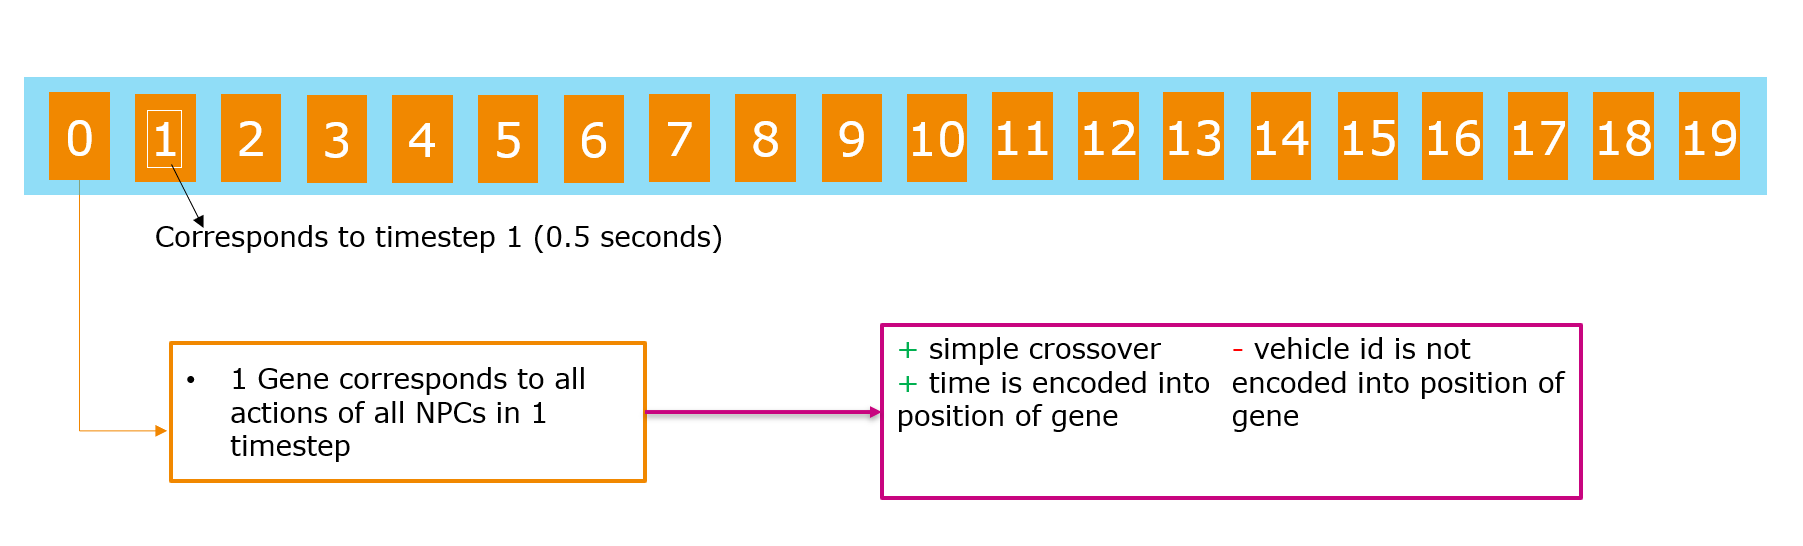
\includegraphics[width=1\linewidth]{figures/time_encoding}
	\caption{Time}
	\label{figure:encoding:chromosome:time}
\end{figure}


Given the previously stated simulation time of 35 seconds, each chromosome has a length of $35 * 2 = 70$ genes.
Crossover can now only move all actions of a time step at once, modifications in the timeline between actions of the same time step will only happen due to a mutation operation.

\paragraph{Time+NPC}
The second encoding is called Time+NPC. Here, one gene corresponds to exactly one action. In order to not loose required information, the ID of each NPC now needs to be encoded into the genes position of its chromosome. One might visualize this as unfolding the matrix build by the genes and chromosome in encoding Time into a linear array. Each actors actions will be listed one after another. Now, each gene has a length of $1$ and each chromosome has a length of $35 * 2 * number\_of\_actors$, which makes them much longer compared to the previous encoding. Figure\ref{figure:encoding:chromosome:time_npc} provides a visualization. In this example, a gene at position 13 corresponds to an action for NPC 2 at time step 3 (which is at 1.5 seconds in the simulation).

\begin{figure}[ht] 
	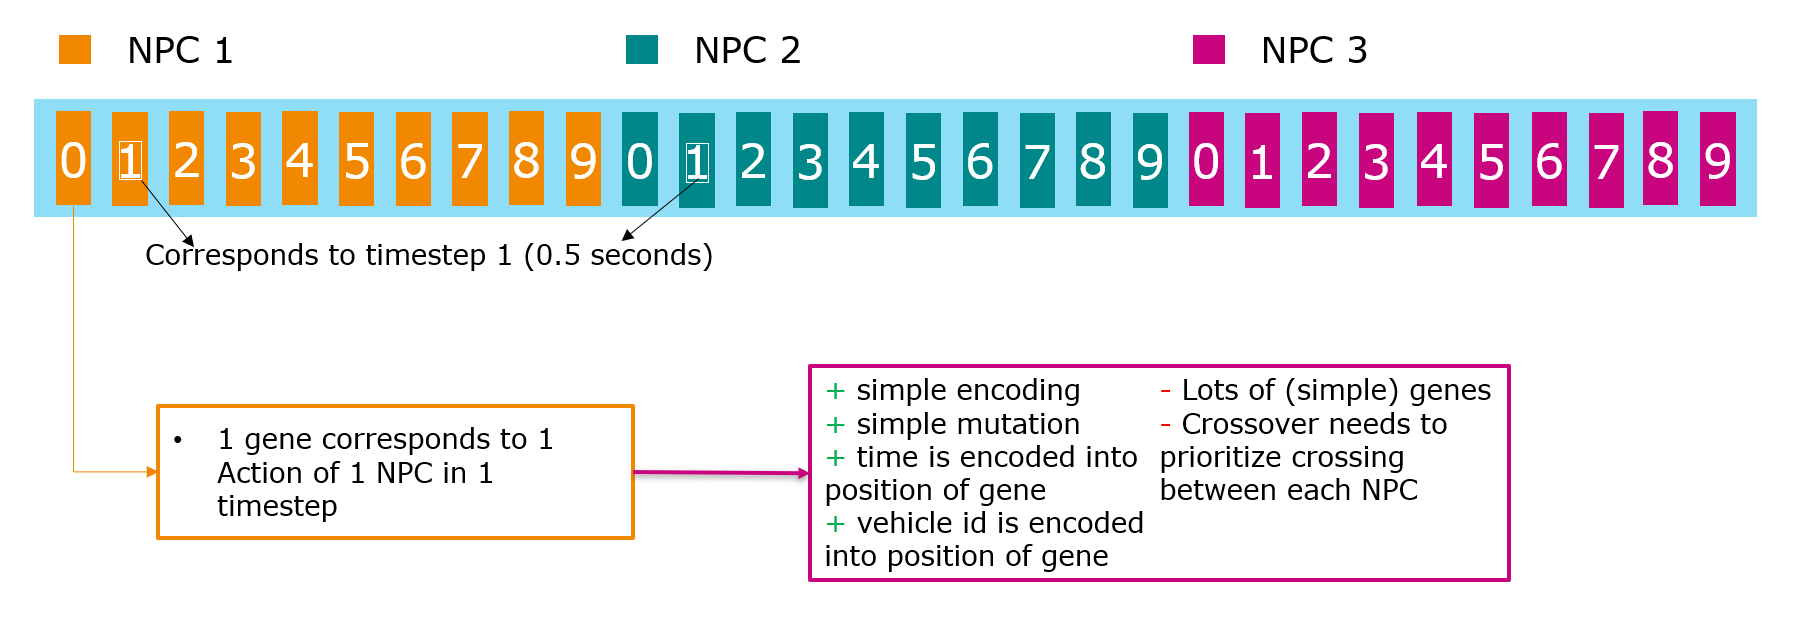
\includegraphics[width=1\linewidth]{figures/time_npc_encoding}
	\caption{Time + NPC}
	\label{figure:encoding:chromosome:time_npc}
\end{figure}

\todo{provide better explaination for crossover}
However for this encoding to make sense, the crossover operations OnePoint and TwoPoint had to be modified. For each NPC, these crossover operations are applied individually. If this was not the case, OnePoint crossover would introduce changes to actions of only one NPC. Because the different crossover points are independently chosen, the position of the crossing differs between the NPCs. This fact allows the crossover operation to break up actions at the same time step, which was not possible with the Time encoding.

\subsubsection{Gene}
Two different encodings for genes were implemented. A gene always consists of a list, which depending on the chromosome type either has a length of $number\_of\_actors$ (in case of Time) or of length 1 (in case of Time+NPC). The following two encodings thus explain the type of object in these lists.

\paragraph{Integer}
\todo{Bad explanation for integer encoding, needs rewriting}
The first encoding uses integer, which are translated into actions when the simulation is started. For each action, a range of integers is assigned, the larger the range, the more likely the action is chosen by the GA. These ranges were assigned based on intuition and trial and error. In Appendix \todo{ref appendix} these probabilities can be viewed.

Actions have parameters split into different ranges, according to which values make sense. For example ModifyTargetVelocity has five different percentages assigned, namely 50, 70, 100, 130, 160. The range of integers assigned to each of these parts is different as well. A percentage setting of 100 for example has the largest integer range assigned.

Actions will be split into 1 or more parts that get an range of integer assigned. Combing these ranges results in a continuos list of integers.
The encoding is visualized in \ref{figure:encoding:gene:int}

\begin{figure}[ht] 
	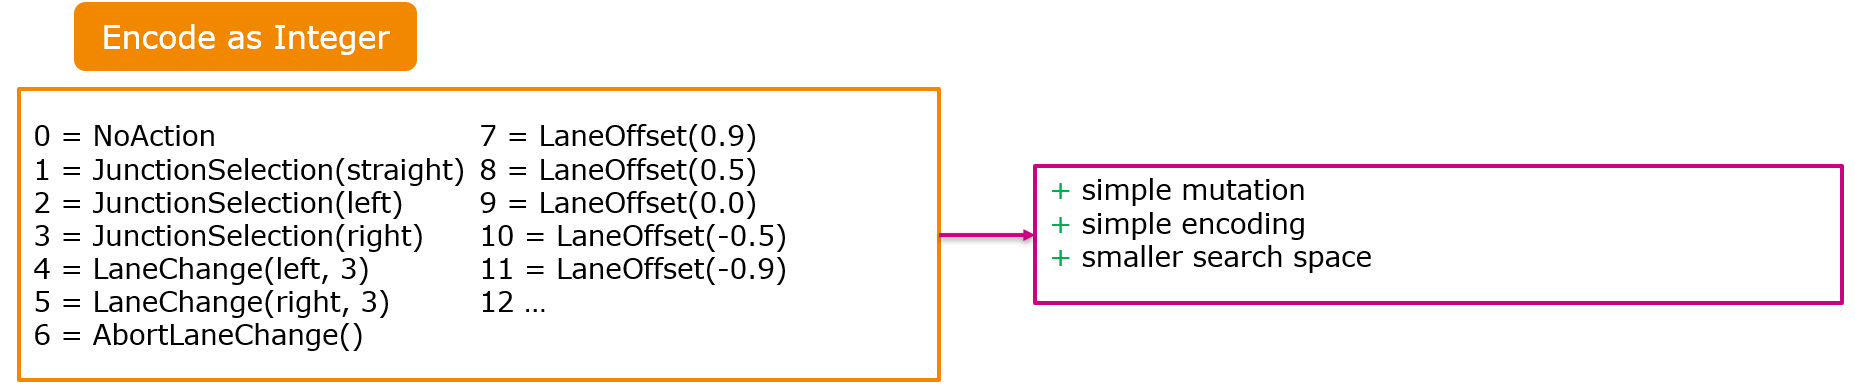
\includegraphics[width=1\linewidth]{figures/int_encoding}
	\caption{Integer}
	\label{figure:encoding:gene:int}
\end{figure}

\paragraph{Dictionary}
\todo{Also bad explanation for dicitinary encoding, needs rewriting}
The second encoding for genes corresponds exactly to the actual actions used in the simulations, requiring no translation. Each action is again selected based on the same probabilities as for the integer encoding\todo{ref appendix}. For actions without parameters, the different encoding will make no difference. However actions with parameters no longer are split into different discrete settings. Now, each parameter is chosen by a randomness function, which is individually selected per action. For example in case of the percentage parameter in ModifyTargetVelocity, the values are selected from a gaussian distribution with mu=100, sigma=25 and a range limit between 0 and 300. Figure \ref{figure:encoding:gene:dict} shows a visualization. Again, these probability functions with settings were assigned based on intuition as well as trial and error. Detailed information can be seen in Appendix \todo{ref appendix}.

\begin{figure}[ht] 
	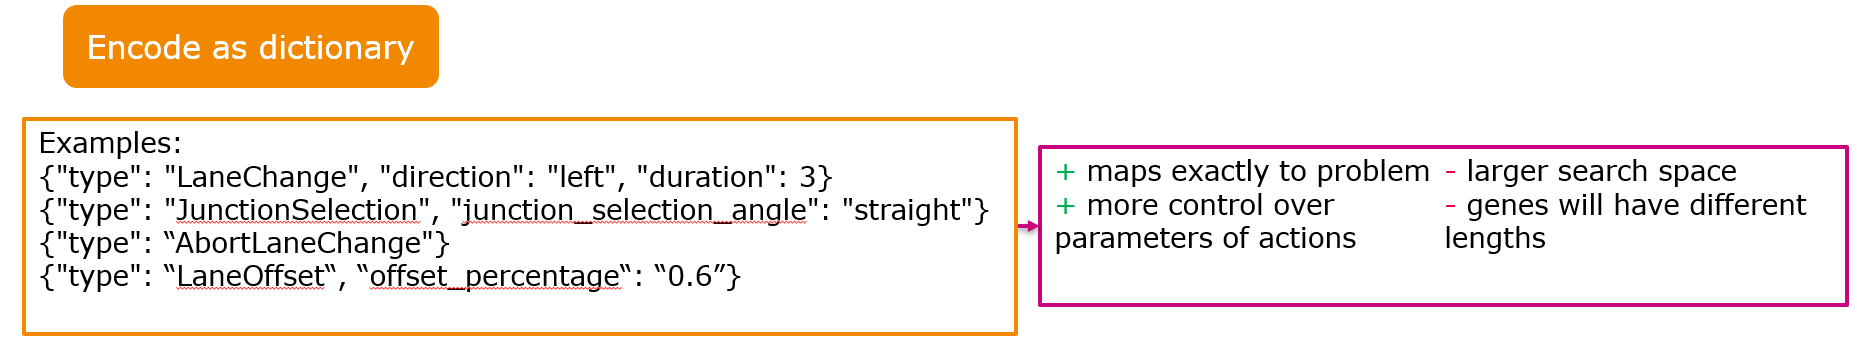
\includegraphics[width=1\linewidth]{figures/dict_encoding}
	\caption{Dictionary}
	\label{figure:encoding:gene:dict}
\end{figure}

Compared to Integer encoding, this method allows for much higher granularity when selecting parameters. If the performance of a genetic algorithm differs between these settings will be investigated in Chapter \ref{chap:hyperparameter_tuning}.

\subsection{Cost Function}
\label{implementation:cost_function}
This master's thesis only utilized internal values from the Traffic Manager for the cost function. Namely if the ego vehicle has to initiate an emergency break. The emergency break values are booleans stored in a list called result["ego\_emergency\_stop"] which has a length of $100 * simulation\_duration\_seconds$ (because of 100hz). 

In case an emergency break lasts longer than 3 seconds, a penalty will be applied. This penalty was introduced as it mitigated results, where the ego vehicle is constantly brake-checked\footnote{\enquote{the unsafe action of applying a car’s brakes to dissuade a driver who is following too closely} according to \href{https://www.dictionary.com/e/slang/brake-check/}{https://www.dictionary.com/e/slang/brake-check/}} by the leading vehicle. The following code snipped shows the cost calculation:\todo{explain code a bit}
\begin{lstlisting}[language=Python, tabsize=4]
SEPS_PER_SECOND = 100
# allow emergency breaks to last only 3 seconds
MAX_DURATION = 3 * STEPS_PER_SECOND

cost = 0
duration_counter = 0
for i in range(len(result["ego_emergency_stop"])):
	if not result["ego_emergency_stop"][i]:
		# base cost in case of no current emergency break
		cost = cost + 1
		duration_counter = 0
	else:
		if duration_counter > MAX_DURATION:
			# increase cost if emergency break max duration is exceeded
			cost = cost + 10
		duration_counter += 1
return cost
\end{lstlisting}

The resulting cost values however are a not easy to interpret, thus these numbers are modified using equation \ref{equ:modified_cost}.

\begin{equation} 
	\label{equ:modified_cost}
	\begin{split}
		cummulated\_emergency\_break\_duration & = (3500 - cost) / 100
	\end{split}
\end{equation}

The constant 3500 is chosen to account for the 100hz sampling rate and the duration of 35 seconds. The division by 100 transforms the value into seconds. This value will be used from now on instead. A higher cumulated emergency brake duration is preferable. It is important to consider, that this value might not exactly correspond to the actual cumulated emergency brake duration time from the simulation, due to the penalty which the cost function applies for emergency breaks that last longer then 3 seconds.

Optimizing for different cost functions, such as improving time to collision (TTC)\todo{explanation} would have been interesting as well. However at the time, no working TTC functionality was implemented. Consequently, only the emergency break cost function will be optimized by the genetic algorithm.

\section{Behaviour Tree}
The EGO vehicle will not be controlled by the genetic algorithm, rather by a behaviour tree. The general idea is to have an EGO vehicle moving in a relatable manner trough the world. It will try to dodge standing or slow moving obstacles. Every 3 seconds the behaviour tree switches between left, straight and right for the junction selection, to produce more interesting scenarios, where the EGO vehicle is not always moving straight. Figure \ref{fig:bt} shows the behaviour tree implemented.

\begin{figure}[ht]
	\label{fig:bt}
	\centering
	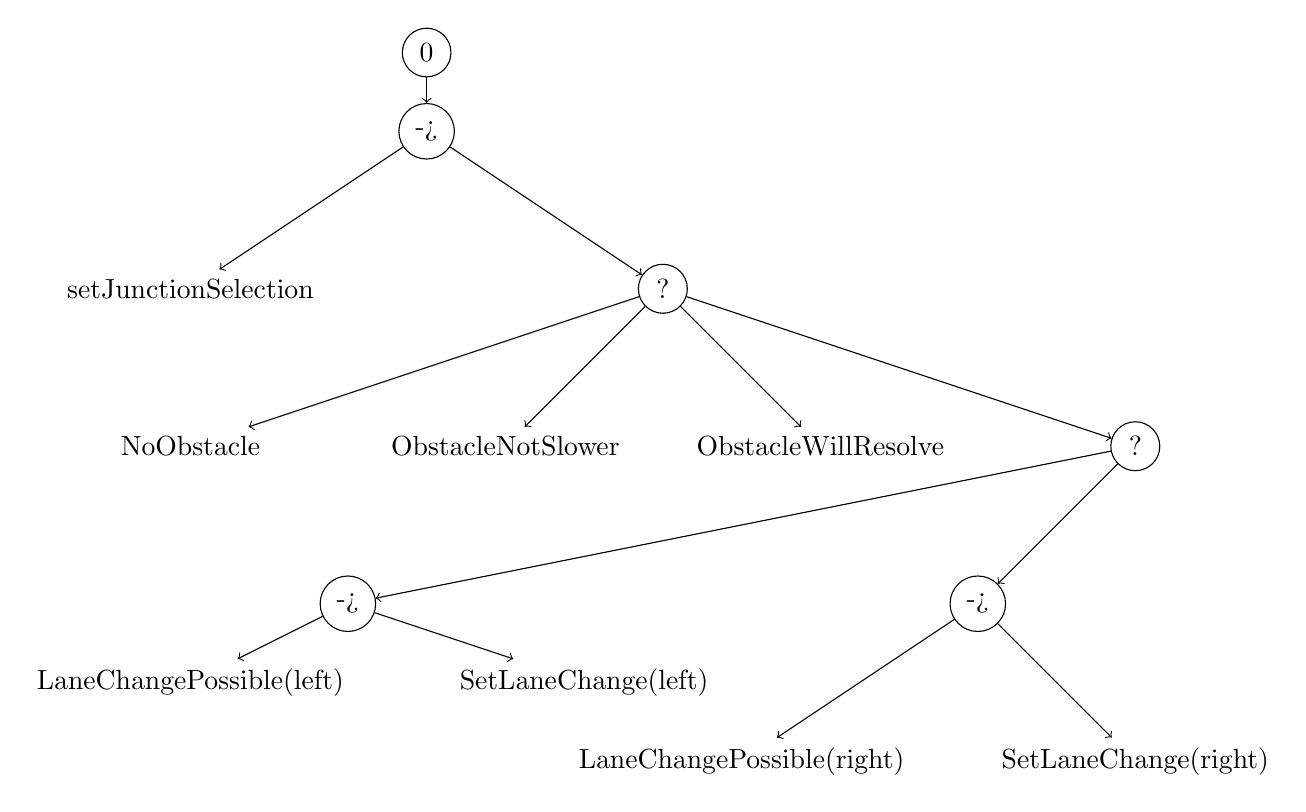
\begin{tikzpicture}
		% Define 1 2 3
		\node[draw, circle] (NodeStart) at (0,0) {0};
		\node[draw, circle] (Sequence1) at (0,-1) {->};
		\draw[->] (NodeStart) -- (Sequence1);
		
		\node (Action1) at (-3,-3) {setJunctionSelection};
		\node[draw, circle] (OR1) at (3,-3) {?};
		\draw[->] (Sequence1) -- (Action1);
		\draw[->] (Sequence1) -- (OR1);
		
		\node (Action21) at (-3,-5) {NoObstacle};
		\node (Action22) at (1,-5) {ObstacleNotSlower};
		\node (Action23) at (5,-5) {ObstacleWillResolve};
		\node[draw, circle] (OR2) at (9,-5) {?};
		\draw[->] (OR1) -- (Action21);
		\draw[->] (OR1) -- (Action22);
		\draw[->] (OR1) -- (Action23);
		\draw[->] (OR1) -- (OR2);
		
		\node[draw, circle] (Sequence31) at (-1,-7) {->};
		\node[draw, circle] (Sequence32) at (7,-7) {->};
		\draw[->] (OR2) -- (Sequence31);
		\draw[->] (OR2) -- (Sequence32);
		
		\node (Action41) at (-3,-8) {LaneChangePossible(left)};
		\node (Action42) at (2,-8) {SetLaneChange(left)};
		\node (Action43) at (4,-9) {LaneChangePossible(right)};
		\node (Action44) at (9,-9) {SetLaneChange(right)};
		\draw[->] (Sequence31) -- (Action41);
		\draw[->] (Sequence31) -- (Action42);
		\draw[->] (Sequence32) -- (Action43);
		\draw[->] (Sequence32) -- (Action44);
		
		
	\end{tikzpicture}
	\caption{Used Behaviour Tree}
\end{figure}
\todo{better visual BT}

While the behaviour tree has access to the same Action Interface (described in section \ref{implementation:action_interface}) as the genetic algorithm, it needs a higher level of integration with the Traffic Manger. The genetic algorithm is only interested in the resulting emergency break values, the behaviour tree however needs access to internal functions during the simulation. Conditions like NoObstacle() or LaneChangePossible() execute internal Traffic Manager functions to get needed information on the world around the EGO vehicle.

\todo{detailed explanation on bt functions}
